\documentclass[../../D1.tex]{subfiles}

\begin{document}

 \begin{figure}[H]
    \begin{center}
        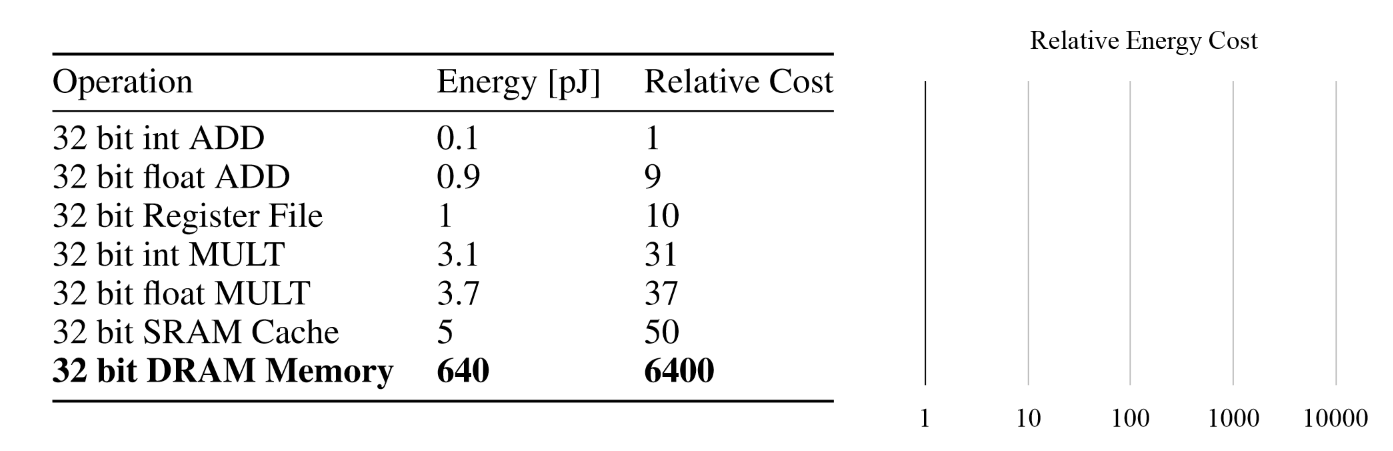
\includegraphics[width=1\textwidth]{45nmCMOSenergyCost.png} 
    \end{center}
    
    \caption{Energy table for 45nm CMOS process\\ \textbf{(Adopted figure from~\autocite{hanLearningBothWeights2015})}}
    \label{fig:45nmCMOS}   
\end{figure}

 The increasing popularity of DNNs for classification tasks such as computer vision, speech recognition and natural language processing has promted work to accelerate execution using specialised hardware. 
 AI accelerators tend to prioritise improving the performance of networks from two perspectives; increasing compuational throughput, and decreasing energy consumption.
 Energy consumption is critical to the feasibility of performing inference on mobile devices, the dominant factor in this area is memory access, figure.~\ref{fig:45nmCMOS} shows the energy consumption for a 32 bit floating point add operation and a 32 bit DRAM memory access on a 45nm CMOS chip, they note that DRAM memory access is 3 orders of magnitude of an add operation.
 Hardware is commonly referred to as an AI accelerator, these can be built to accelerate both the \emph{training} and \emph{inference} stages of execution, this section will specifically focus on the \emph{inference} phase, however some of the following are capable of both.

\subsubsection{GPU}

\subsubsection{VPU}
One commercial hardware accelerator using a VPU architecture is the Intel Movidius Neural Compute Stick.
\begin{itemize}
    \item 16 VLIW (very long instruction word) SHAVE (streaming hybrid architecture vector engine) processors, optimized for machine vision and able to run parts of a neural network in parallel
    \item 4Gb LPDDR3 DRAM
\end{itemize}

\begin{figure}
    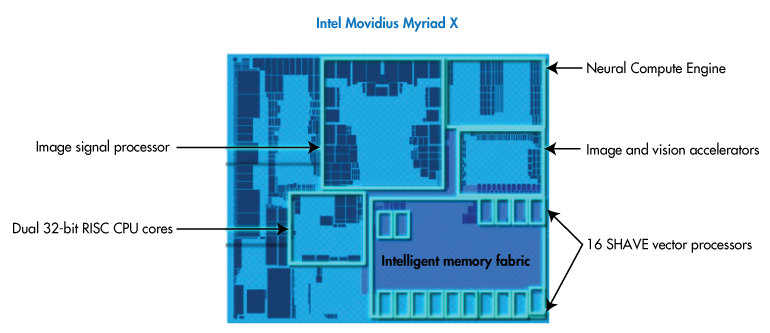
\includegraphics[width=1\textwidth]{movidius-myriad-x.png}
    \caption{High level view of the Intel Movidius Myriad X VPU}
    \label{fig:MyriadX}
\end{figure}

\subsubsection{TPU}
The \acrshort{tpu} is a custom \acrshort{asic} developed by google, designed specifically for TensorFlow, conventional access to these chips is via a cloud computing service. 
Google claims~\autocite{GoogleWinsMLPerf}~the latest 4th generation TPUv4 is capable of more than double the matrix multiplication TFLOPs of TPUv3 (Wang et al.~\autocite{wangBenchmarkingTPUGPU2019}~describes a peak of 420 TFLOPs for the TPUv3).
The TPU implements data parallelism in a manner prioritising batch size, one batch of training data is split evenly and sent to each core of the TPU, so total on-board memory determins the maximum data batch size.
Each TPU core has a complete copy of the model in memory, so the maximum size of the model is determined by the amount of memory avaliable to each core~\autocite{wangBenchmarkingTPUGPU2019}.



\end{document}